\documentclass
[10pt, xcolor=dvipsnames]
%[11pt,compress ,xcolor=dvipsnames]
{beamer}

\usepackage{graphicx}
\graphicspath{ {../figures} }

\usepackage{caption}
\captionsetup[figure]{font=scriptsize,labelfont=scriptsize}
\captionsetup[table]{font=scriptsize,labelfont=scriptsize}

% justified text
\renewcommand{\raggedright}{\leftskip=0pt \rightskip=0pt plus 0cm}

% overlays
%\setbeamercovered{transparent}

% bibliography 

\usepackage[utf8]{inputenc}
\usepackage[english]{babel}
%\usepackage[
%    style=alphabetic, 
%    backend=bibtex,
%    sorting=none
%    ]{biblatex}
%\bibliography{ref}{}
%\renewcommand*{\bibfont}{\scriptsize}

% Removes icon in bibliography
%\setbeamertemplate{bibliography item}{\hspace{-4em}}

\usepackage{amsmath}
\usepackage{braket}
\usepackage{booktabs}
\usepackage{tikz}
\usepackage{adjustbox}
\usepackage{verbatim}
\usepackage{setspace}
\usepackage{subcaption}

\usepackage[] %qm
{qcircuit}
% theme


\useoutertheme[]{infolines} % Alternatively: miniframes, infolines, split
%\usecolortheme{whale}
%\usetheme{CambridgeUS}
\useinnertheme{circles}
%
\definecolor{UBCblue}{rgb}{0.04706, 0.13725, 0.26667} % UBC Blue (primary)
\definecolor{UBCgrey}{rgb}{0.3686, 0.5255, 0.6235} % UBC Grey (secondary)
\definecolor{light-grey}{RGB}{240,240,240}

\setbeamercolor{palette primary}{bg=UBCblue,fg=white}
\setbeamercolor{palette secondary}{bg=UBCblue,fg=white}
\setbeamercolor{palette tertiary}{bg=UBCblue,fg=white}
\setbeamercolor{palette quaternary}{bg=UBCblue,fg=white}
\setbeamercolor{structure}{fg=UBCblue} % itemize, enumerate, etc
\setbeamercolor{section in toc}{fg=UBCblue} % TOC sections
\setbeamercolor{subsection in head/foot}{bg=UBCgrey,fg=white}
\setbeamercolor{title}{bg=UBCblue,fg=white}
\setbeamercolor{block title}{bg=UBCgrey,fg=white}
\setbeamercolor{block body}{bg=light-grey, fg=black}
\setbeamercolor{frametitle}{bg=light-grey,fg=black}


% ------- DOCUMENT --------

\title[The pizza guy]{The pizza guy problem using Minizinc}
\author[Boldini, Diana, Zaglio]{G. Boldini, A. Diana, F. Zaglio}
\institute[UNIPR]{University of Parma\newline
    Master's Degree in Computer Science\newline
    Constraint Programming}
\date{AA 2021/22}


\newcommand\blfootnote[1]{%
  \begingroup
  \renewcommand\thefootnote{}\footnote{#1}%
  \addtocounter{footnote}{-1}%
  \endgroup
}


\AtBeginSection[]{
	\begin{frame}{Outline}
		\tableofcontents[sectionstyle=show/shaded,subsectionstyle=show/shaded/hide,subsubsectionstyle=show/shaded/hide]
	\end{frame}
}



\begin{document}

% interlinea
%\linespread{1.5}
%\doublespacing


\setbeamertemplate{navigation symbols}{}


% title 
\begin{frame}[plain]
    \titlepage
\end{frame}
\addtocounter{framenumber}{-1}


% outline
\begin{frame}{Outline}
    \tableofcontents[sectionstyle=show,subsectionstyle=show/shaded/hide,subsubsectionstyle=show/shaded/hide]
%    \tableofcontents
\end{frame}


\section{Introduction}

\begin{frame}[allowframebreaks]
    {The pizza guy problem}
    The best pizzeria in the town delivers pizzas at home and we want to find:
    \begin{itemize} 
        \item the best schedule of the set of orders,
        \item minimize the total traveled distance by all the deliverers, 
        \item respect the delivery times requested by the customers.
    \end{itemize}
    \vspace{0.3cm}
    Solving the problem means:
    \begin{itemize}
        \item assign a set of sorted lists of orders to every deliverer,
        \item where each list represents an "ordered" travel.
    \end{itemize}
    \pagebreak
    \begin{enumerate}
		\item An \textit{order} consists in:
		\begin{enumerate}
			\item a delivery address,
			\item a desired delivery time (granularity of 15 minutes) from 19.00 to 22.00,
			\item a number of pizzas.\\~\
		\end{enumerate}
        \item Delivery window:
        \begin{enumerate}
			\item is up to 30 minutes later than desired delivery time;
			\item during this time, multiple travels from and to the pizzeria are allowed.\\~\
		\end{enumerate}

		\item The street topology of the city can be seen as a graph (the edges rappresent the travel time).\\~\
		\item Max pizza carried by a deliverer: 16.
		
	\end{enumerate}
\end{frame}

\section{Model}
\begin{frame}{Input Data}
    The input consists in having:
	\begin{enumerate}
		\item $d$: number of deliverers,
		\item $mdist$: 2-d matrix representing the travel distance between
			every pair of nodes (with Dijkstra),
		\item $k$: side dimension of $mdist$,
		\item a set of $N$ orders, each of them made by a destination $dest$, a delivery 
			time $orario$ and a number of pizzas $num\_pizzas$:
            
			\begin{equation*}
				\begin{split}
					\text{orario} &= [o_1, o_2, \dots, o_N];\\
					\text{num\_pizzas} &= [np_1, np_2, \dots, np_N];\\
					\text{dest} &= [d_1, d_2, \dots, d_N];
				\end{split}	
			\end{equation*}
	\end{enumerate}
\end{frame}
\begin{frame}{Assumptions}
	\begin{enumerate}
		\item the graph could be undirected;\\~\
		\item a deliverer can do only a single travel 
        (from pizzeria, to all destination nodes and back to pizzeria) in one half-an-hour ($h$);
        \begin{itemize}
            \item the total number of $h$ is 6 (\# slots in 19.00 - 22.00)\\~\
        \end{itemize}
            
		\item distances and travels time are considered the same thing;\\~\
		\item the set of orders is known before the start of the evening;\\~\
		\item all the time needed by the deliverer to interacts with customers
                 is supposed to be zero. 
	\end{enumerate}
\end{frame}

\begin{frame}[allowframebreaks]{Implementation}
    $d$ : \# deliverers, $N$: \# deliveries and $h$: \# time slots.\\~\

    As decisional variables, we used these following data structures:
    \begin{itemize}
		\item {scheduling:\\
            \begin{center}
                \texttt{array[1..d, 1..N, 1..h] of var bool: scheduling;}
            \end{center}    
        }
        \item {P: destinations to reach\\
            \begin{center}
                \texttt{array[1..d, 1..N, 1..h] of var array2set(dest) union {0}: P;}
            \end{center}
        }
		\item {X: position of destinations to reach\\
            \begin{center}
                \texttt{array[1..d, 1..N, 1..h] of var 0..N: X;}
            \end{center}
        }
        \item {distances\\
            \begin{center}
                \texttt{array[1..d, 1..N, 1..h] of var 0..29: distances;}
            \end{center}
        }
        \pagebreak
		\item {pizza\_carried\\
            \begin{center}
                \texttt{array[1..d, 1..h] of var 0..16: pizzas\_carried;}
            \end{center}
        }
		\item {estimated arrival (ea)\\
            \begin{center}
                \texttt{array[1..N] of var 0..h*30: ea;}
            \end{center}
        }
		
		\item {total\_travel\\
            \begin{center}
                \texttt{array[1..d, 1..h] of var 0..29: total\_travel;}
            \end{center}
        } 
	\end{itemize}
\end{frame}

\begin{frame}[fragile]{Constraints: scheduling and P consistency}
    Scheduling consistency:
    \begin{itemize}
		\item ensures that all the orders are fulfilled: \\
            \begin{center}
                \texttt{sum(scheduling) = N;}
            \end{center}
            
		\item ensures that only one delivever takes care of one order:
          \begin{center}
            \texttt{forall(j in 1..N)(\\
			    sum([scheduling[id,j,ih]| id in 1..d, ih in 1..h]) = 1\\
		  );}
        \end{center}
        \end{itemize}
    \vspace{0.5cm}
    P construction: 
    \begin{verbatim}
    forall(id in 1..d, iN in 1..N, ih in hra[iN])(
        P[id, iN, ih] = scheduling[id, iN, ih] * dest[iN]
    );
    \end{verbatim}
\end{frame}

\begin{frame}[fragile]{Constraints: X consistency}
    X has to contain all the meaningful positions in P:
    \begin{verbatim}
    forall(id in 1..d, iN in 1..N, ih in 1..h)(
        if P[id, iN, ih] > 0 then 
            count([ X[id, iNN, ih] | iNN in 1..N], iN, 1)
        else
        (
            count([ X[id, iNN, ih] | iNN in 1..N], iN, 0) 
            /\
            distances[id,iN,ih] = 0
        )
        endif
    );
    \end{verbatim}
    Also, for each row of X, we want to push all the meaningless values (zeros) to the end
    (done in another constraint).
\end{frame}

\begin{frame}[fragile]{Constraints: distances calculation}
    Considering a single row of \texttt{X}, two different cases:
    \begin{itemize}
        \item the first (meaningful) cell;
        \item all the others (meaningful) cells.
    \end{itemize}
\begin{verbatim}
    forall(id in 1..d, iN in 1..N, ih in 1..h)(
        if X[id,iN,ih] !=0 then
           if iN == 1 then
              distances[id, X[id,iN,ih], ih] = 
                 mdist[1, P[id, X[id,iN,ih], ih]] 
            else
               distances[id, X[id,iN,ih], ih] = 
                 mdist[P[id, X[id,iN-1,ih], ih], P[id, X[id,iN,ih], ih]] 
                  + distances[id,X[id,iN-1,ih], ih]
                       | iNN in 1..iN-1])
            endif
        endif
     );
\end{verbatim}

\end{frame}

\begin{frame}[fragile]{Constraints: total travel}
    
    Total travel consistency ensured by \texttt{total\_travel} domain of \texttt{[0..29]}:
    
    \begin{verbatim}
    constraint forall(id in 1..d, iN in 1..N, ih in 1..h)(
        ( X[id,iN,ih] !=0
            /\ ( iN+1 == N+1 \/ X[id,iN+1,ih] == 0)
            /\ P[id,X[id,iN,ih],ih] != 0)

            -> (total_travel[id,ih] = 
                distances[id, X[id,iN,ih], ih] 
                + mdist[P[id, X[id,iN,ih], ih],1])   
    );
    \end{verbatim}

    
\end{frame}

\begin{frame}[fragile]{Constraints: ea \& pizza\_carried}

Expected arrival: all the orders must arrive in the delivery window.
    \begin{verbatim}
forall(iN in 1..N)(
   ea[iN] = sum([scheduling[id,iN,ih]
            * (distances[id,iN,ih]+((ih-1)*30)) 
               | id in 1..d, ih in 1..h])
   /\ ea[iN] >= ra[iN] 
   /\ ea[iN] < ra[iN]+30 
);
    \end{verbatim}

Number of pizzas carried for each travel:
    \begin{verbatim}
forall(id in 1..d, ih in 1..h)(
   pizzas_carried[id, ih] = sum([ num_pizze[j]
                                | j in 1..N 
                                where scheduling[id, j, ih] = 1])
);
    \end{verbatim}
\end{frame}


\begin{frame}{Graphical representation}

    \begin{center}
        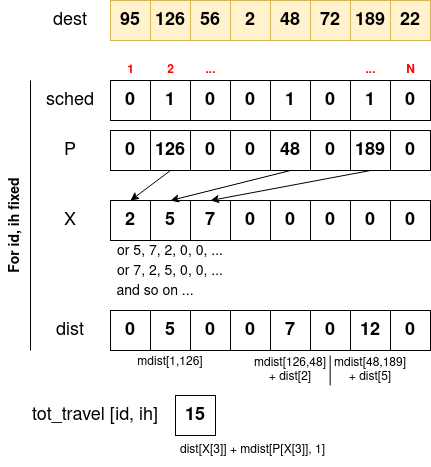
\includegraphics[scale=.45]{drawio.png}
    \end{center}

\end{frame}

\begin{frame}[fragile]{Restrict the search space}

    \begin{enumerate}
        \item domain restrictions;
        \item for each order, exclude all the non-possible half-an-hour;
        \begin{verbatim}
    forall(id in 1..d, iN in 1..N, ih in (1..h diff hra[iN]))(
        scheduling[id,iN,ih] = 0
        /\ P[id,iN,ih] = 0
        /\ distances[id,iN,ih] = 0
        /\ count( [X[id,iNN,ih] | iNN in 1..N], iN, 0)
    );
        \end{verbatim}
        \item enforce useless cells of \texttt{X} to be zero (and push them to the bottom).
  \begin{verbatim}
    forall(id in 1..d, ih in 1..h)(
        let {
            var int: c = count([P[id,iNN,ih] | iNN in 1..N],0)
        } in forall(iN in N-c+1..N)(
            X[id,iN,ih] = 0
            )
    );
  \end{verbatim}
\end{enumerate}

\end{frame}

\begin{frame}[fragile]{Symmetry breaking}

    Simmetry $\rightarrow$ having multiple deliveriers.\\~\

    \textit{e.g.} 3 orders, 2 deliverers (\texttt{d1} and \texttt{d2}).\\
    \hspace{1em}best strategy: first two togheter, third alone.\\

    \hspace{1em}$\rightarrow$ first two can be assigned to \texttt{d1} and the third to \texttt{d2}\\
    \hspace{2em} and \textbf{viceversa}. \\~\

Impose an order on the deliverers:

\begin{verbatim}
forall(ih in 1..h, id in 1..d-1)(
    pizzas_carried[id,ih] >= pizzas_carried[id+1,ih]
);
\end{verbatim}

\end{frame}

\section{Results}


\begin{frame}{Tests and results}
    

    Different analyzes:
    \begin{itemize}
        \item search strategies comparison;
        \item same problem with different cities (of increasing size);
        \item same city, increasing complexity of the problem;
        \item real-world application.\\~\
    \end{itemize}

    5 real-world italian cities considered:
    \begin{table}[h]
		\centering
		\begin{tabular}{l|ll}
			City & nodes & edges \\
			\hline
			Visano & 297 & 378 \\
			Asola & 480 & 664 \\
			Montichiari & 1130 & 1509 \\
			Brescia & 3925 & 5464 \\
			Roma & 4729 & 7277 \\
		\end{tabular}		
	\end{table}
	
    \texttt{mdist} computed using Dijkstra as pre-preprocessing step.


\end{frame}




\begin{frame}{Search strategies comparison}

    \begin{center}
		$N = 12$ (orders), $d = 2$ (deliverers), city = Visano.	\\~\	
	\end{center}

    Changing the search annotations:
    \begin{itemize}
        \item the search variable;
        \item how the variable is choosen (VCA);
        \item how to constraint the variable (VSA).\\~\
    \end{itemize}

    Results:
    \begin{itemize}
        \item searching of variable \texttt{scheduling} is usually faster;
        \item some VCA (Value Choice Annotation) and
        VSA (Variable Selection Annotations) appear to be more promising 
        than others.
    \end{itemize}
\end{frame}

\begin{frame}{Search strategies comparison: preliminary analysis}
    \begin{figure}
		\centering

		\begin{subfigure}[b]{.3\textwidth}
			\centering
			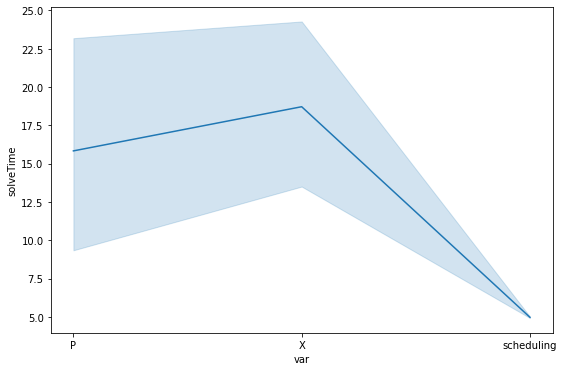
\includegraphics[width=\textwidth]{var.png}
			\caption{changing search variable.}
		\end{subfigure}
		\begin{subfigure}[b]{.69\textwidth}
			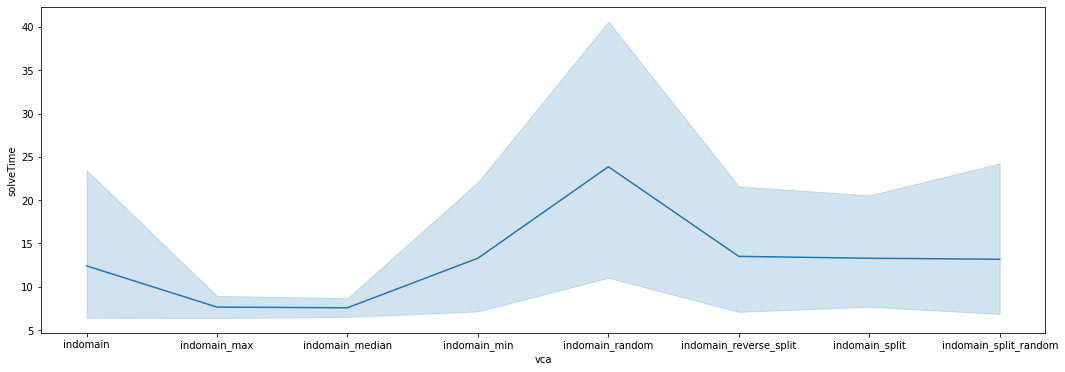
\includegraphics[width=.9\textwidth]{vca.png}
			\caption{changing Value Choice Annotation (VCA)}
		\end{subfigure}
		\begin{subfigure}[b]{\textwidth}

            \centering
            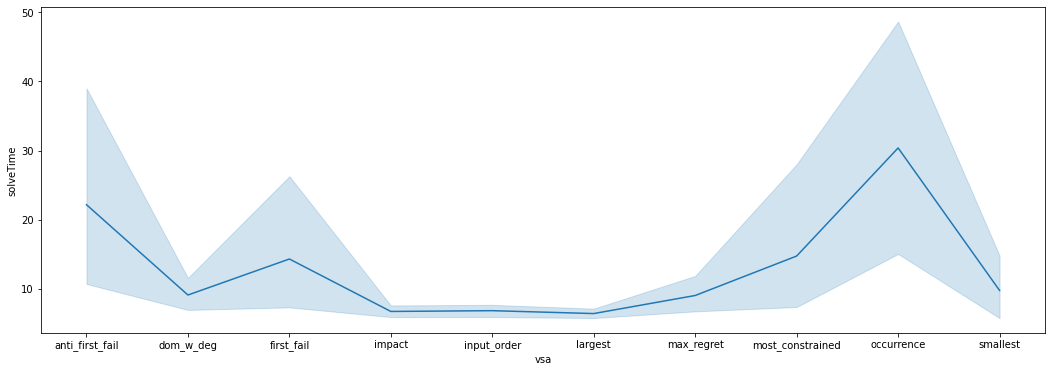
\includegraphics[width=.8\textwidth]{vsa.png}
			\caption{changing Variable Selection Annotations (VSA)}
		\end{subfigure}
		
	\end{figure}
 
\end{frame}

   
    %\includegraphics{}{var.png}



\begin{frame}[allowframebreaks]{Search strategies comparison: more specific analysis}

    Subset of search strategies (the most promising) considered.\\
    Timeout of 20 seconds.\\~\

    Correlation matrix:
    \begin{itemize}
        \item number of failures and number of nodes (1)
        \item number of propagations and solve time (0.79) and 
        non-correlation between maximum depth and solve time (-0.05)
    \end{itemize}

    \begin{figure}
        \centering
        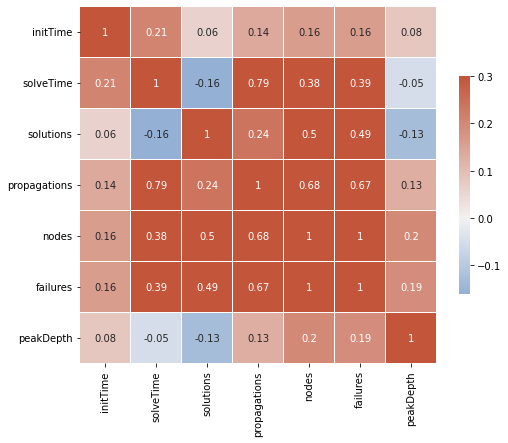
\includegraphics[width=.3\textwidth]{corr.png}
    \end{figure}

    \framebreak

    \begin{figure}
		\centering
		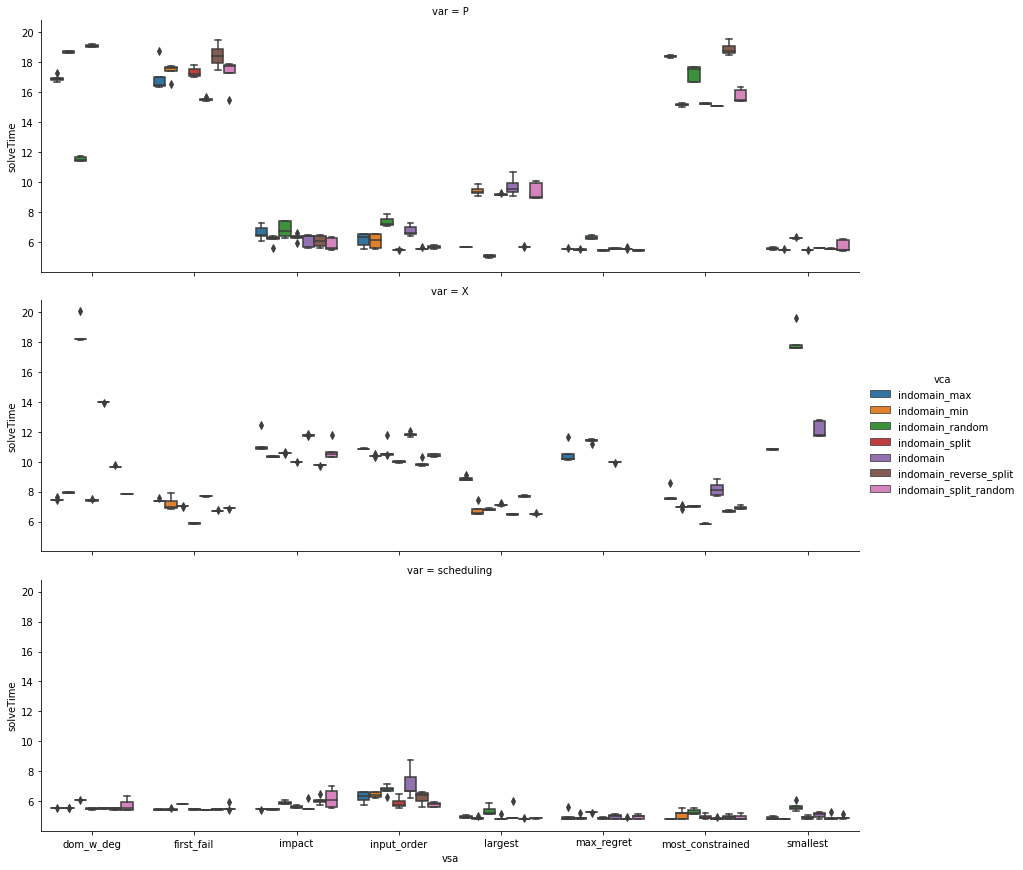
\includegraphics[width=.72\textwidth]{solve-time-specific.png}
	\end{figure}

\end{frame}

\begin{frame}{5 city of increasing size}

    \begin{center}
		$N = 12$ (orders), $d = 2$ (deliverers), changing the city
	\end{center}


    \begin{figure}
		\centering
		\begin{subfigure}[c]{.49\textwidth}
			\centering
			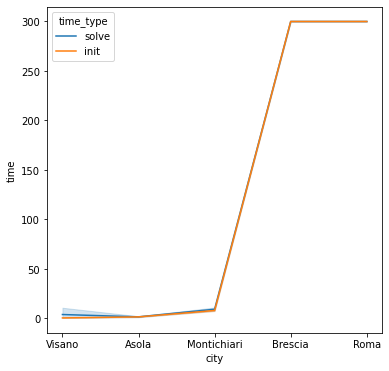
\includegraphics[width=.7\textwidth]{city-increasing-size.png}
		\end{subfigure}
		\begin{subfigure}[c]{.49\textwidth}
			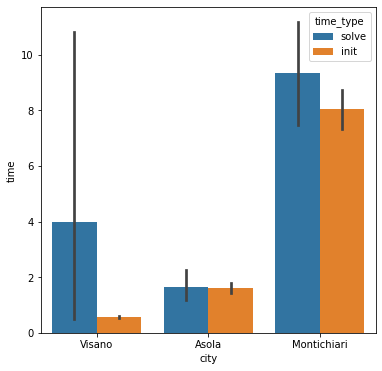
\includegraphics[width=.7\textwidth]{city-increasing-size-2.png}

		\end{subfigure}
	\end{figure}

    Roma and Brescia always reach timeout.

\end{frame}

\begin{frame}[allowframebreaks]{Changing the complexity of the problem}

    $N = 2\dots15,\hspace{.5em} d=1\dots4$, city = Visano, 2 minutes timeout.\\~\

    \begin{figure}
        \centering
		\begin{subfigure}[c]{\textwidth}
            \centering
			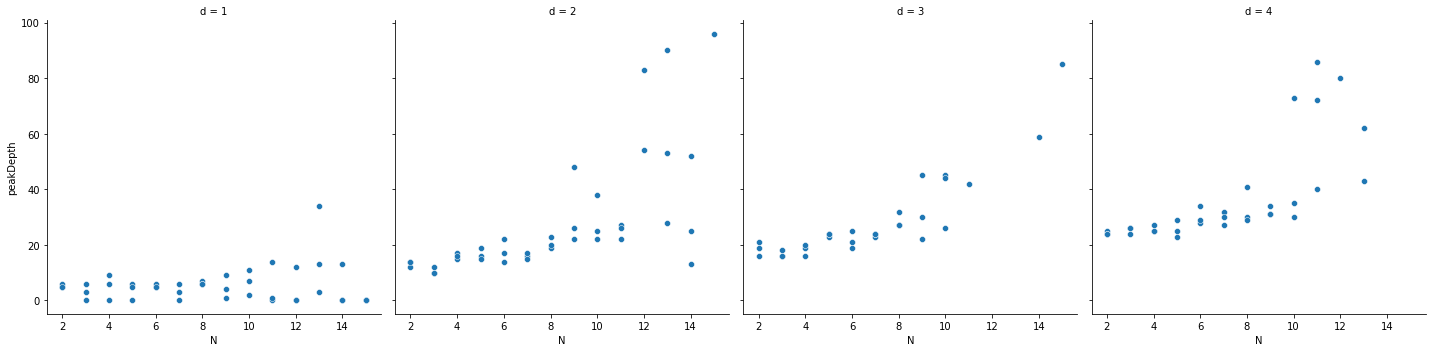
\includegraphics[width=.8\textwidth]{incr-problem-depth.png}
			\caption{peakDepth}
		\end{subfigure}
		\begin{subfigure}[b]{\textwidth}
            \centering
			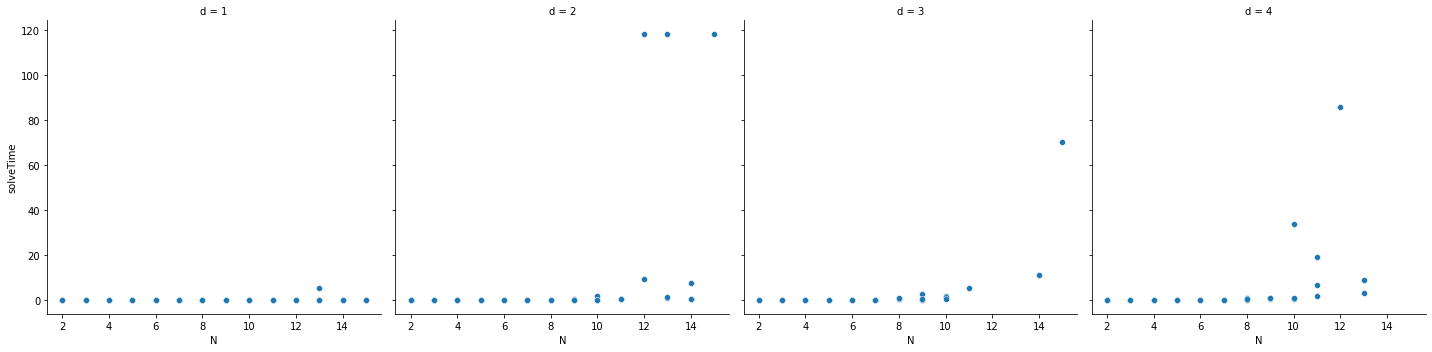
\includegraphics[width=.8\textwidth]{incr-problem-time.png}
			\caption{Solve time}
		\end{subfigure}
		\begin{subfigure}[b]{\textwidth}
            \centering
			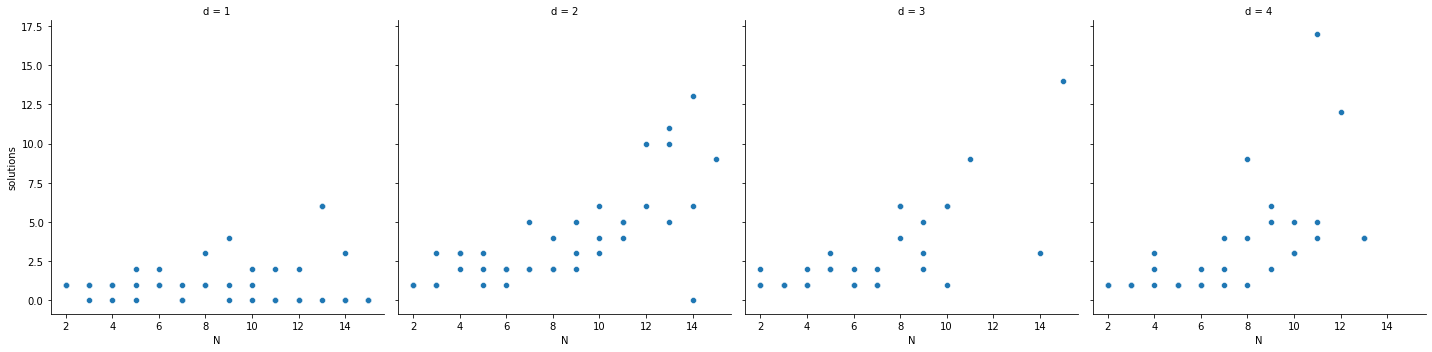
\includegraphics[width=.8\textwidth]{incr-problem-solutions.png}
			\caption{Solutions}
		\end{subfigure}
		\begin{subfigure}[b]{\textwidth}
            \centering
			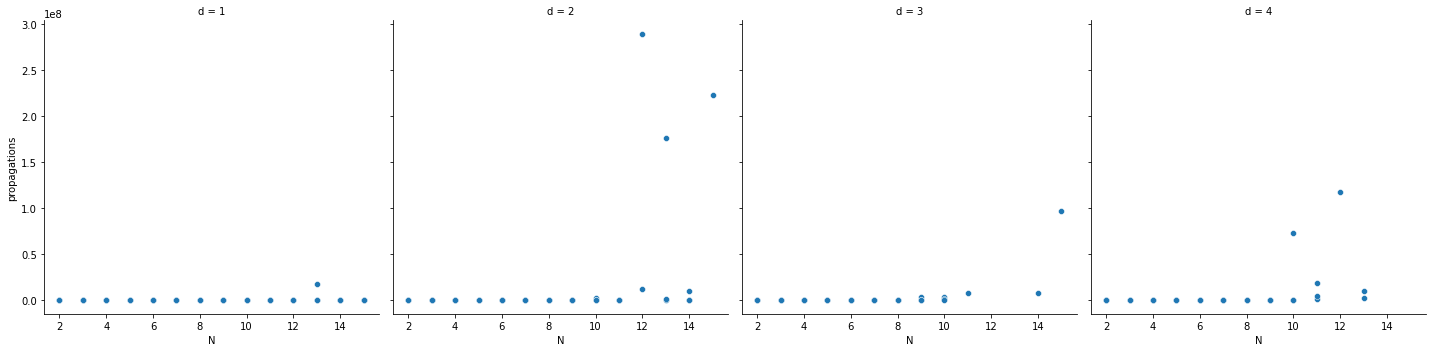
\includegraphics[width=.8\textwidth]{incr-problem-propagations.png}
			\caption{Propagations}
		\end{subfigure}

	\end{figure}
\end{frame}

\begin{frame}{Real world application}

    City graph from \texttt{OpenStreetMap (Python)}.\\
    \texttt{mdist} filled with Dijkstra.\\~\

    \begin{figure}
		\begin{subfigure}[t]{.5\textwidth}
			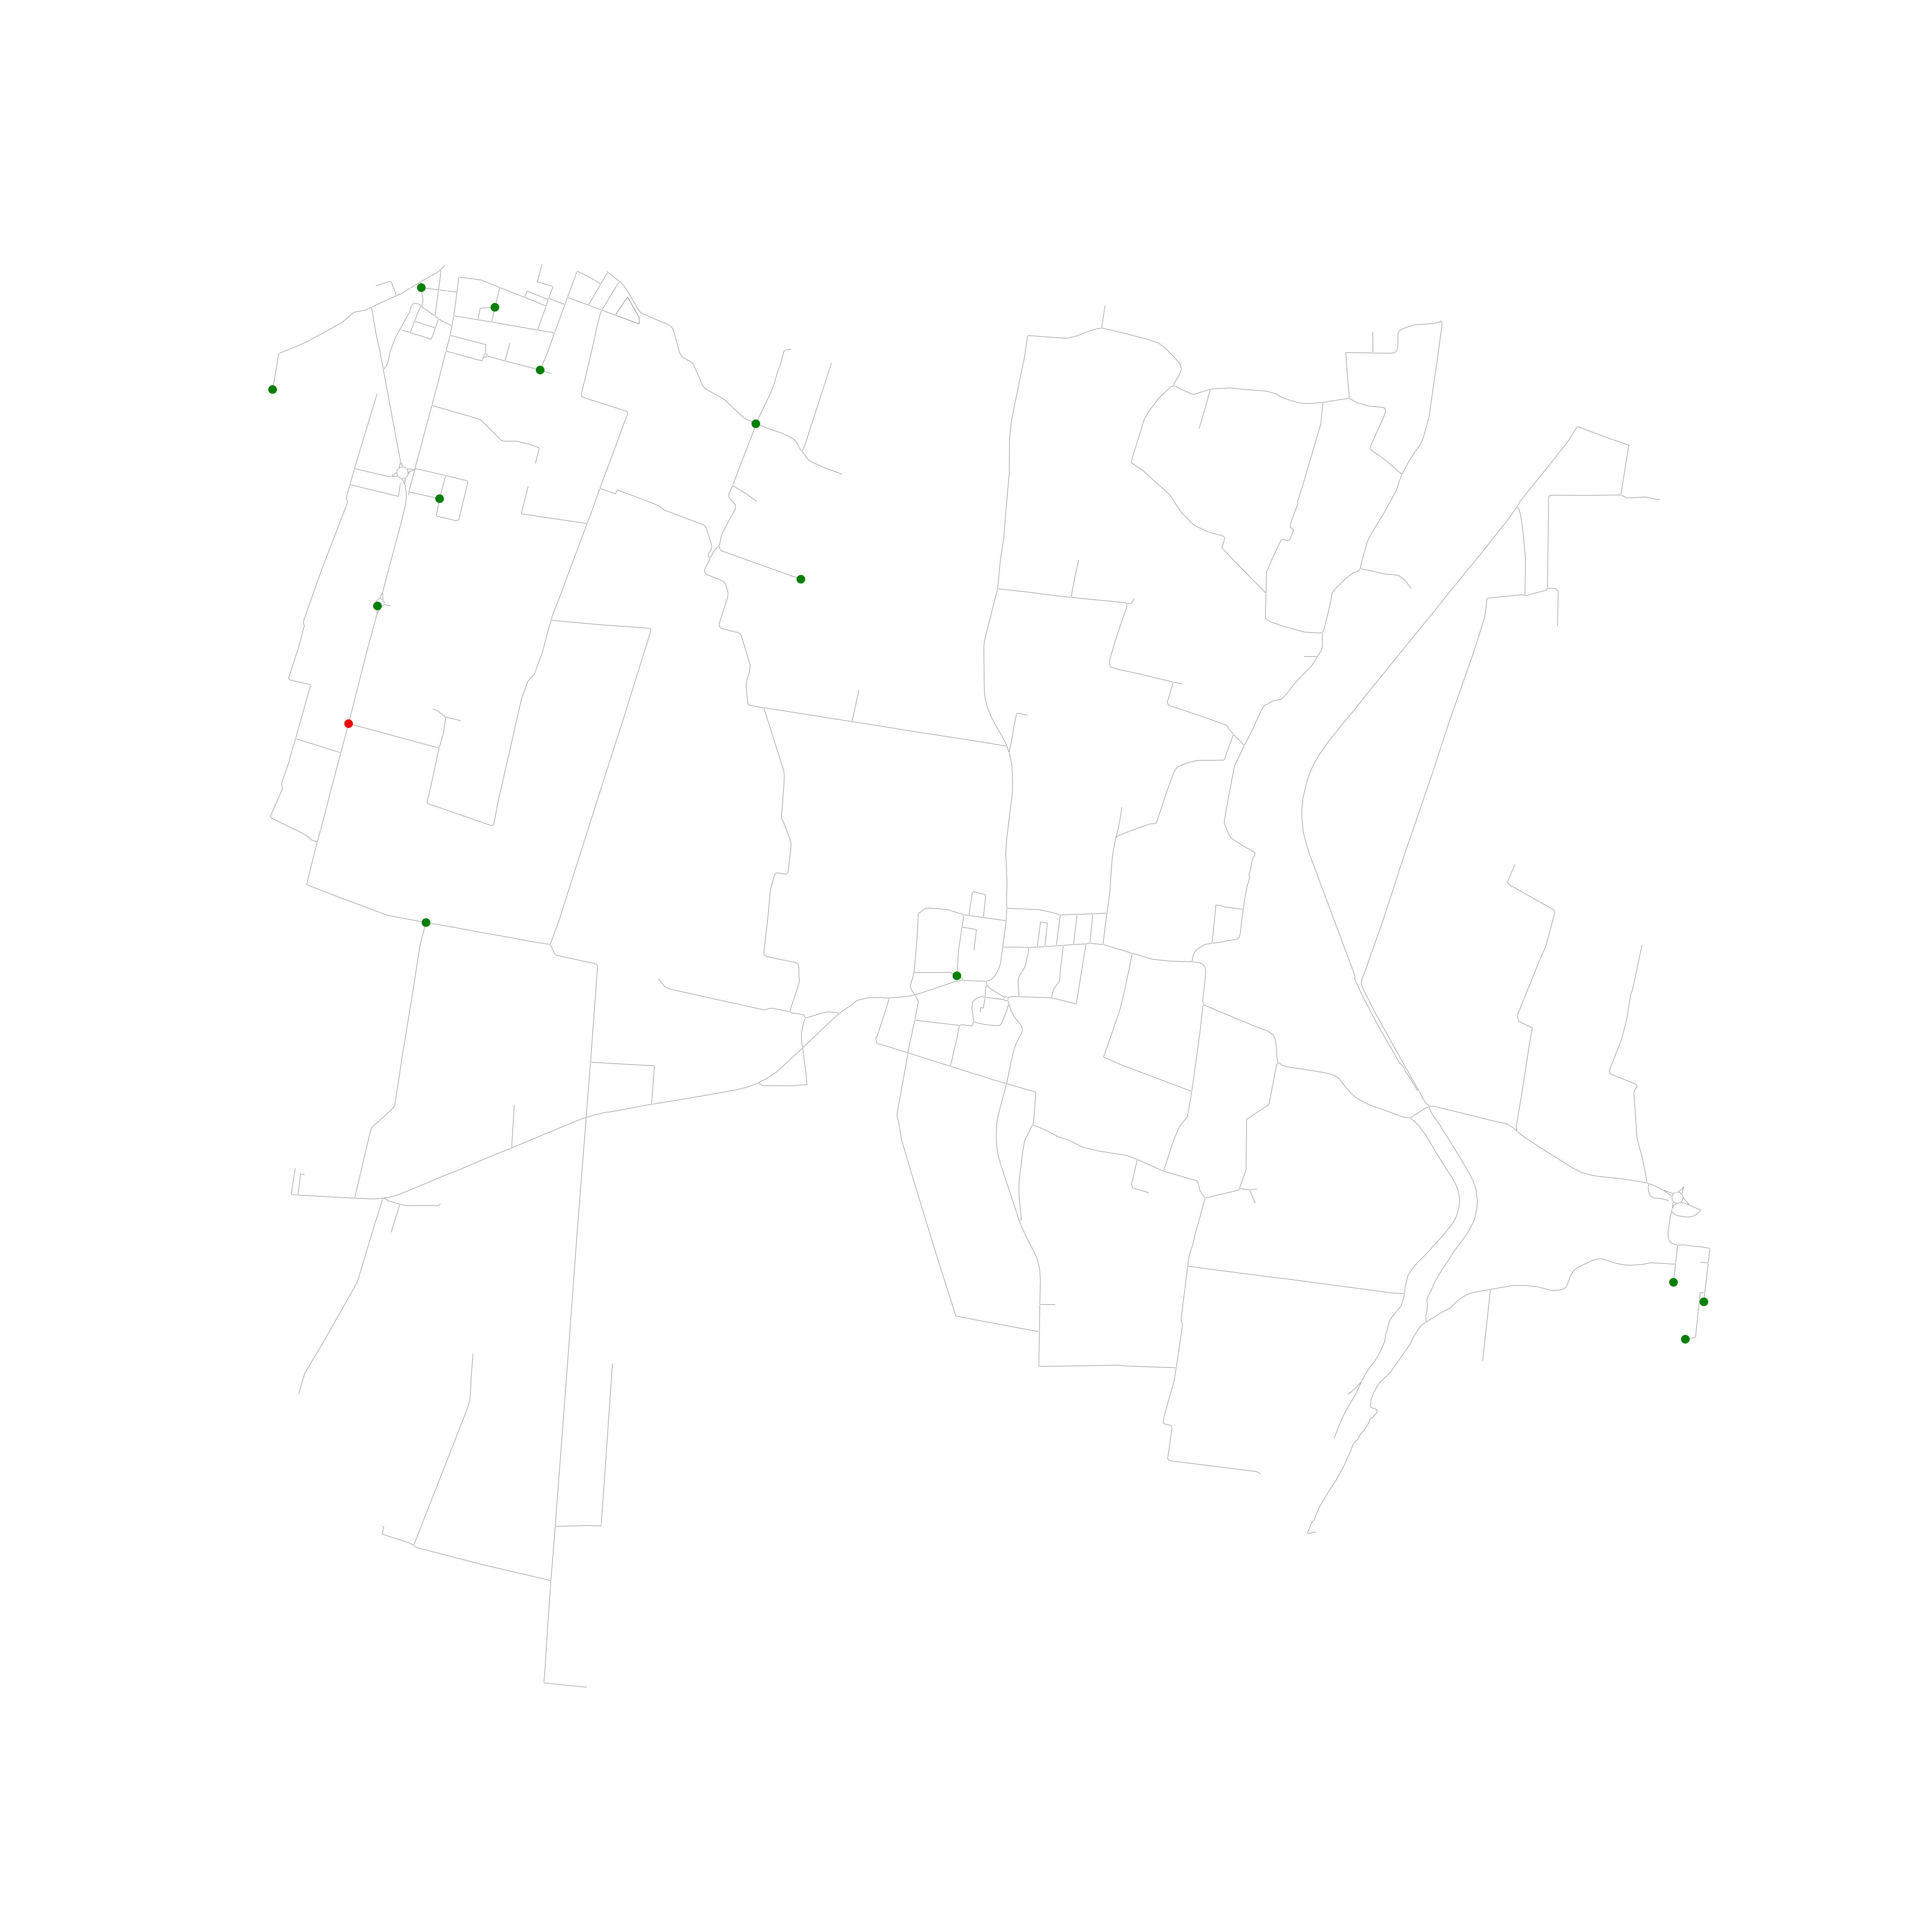
\includegraphics[width=.7\textwidth]{graph.png}
			\caption{Pizzeria (red) and destinations to reach (green)}

		\end{subfigure}
		\begin{subfigure}[t]{.49\textwidth}
			\includegraphics[width=.7\textwidth]{graph_paths-min.png}
			\caption{Path for each deliverer}
		\end{subfigure}
	\end{figure}



    \textit{Visano}, $N = 13$, $d = 2$, solve time: 48.8 seconds.

\end{frame}

\section{Conclusions}

\begin{frame}{Conclusions}
    \begin{enumerate}
        \item Our proposed model seems to work.\\~\
        \item \textit{But} the time increases quickly with the size of the problem:
        \begin{itemize}
            \item timeout of 5 minutes for $N \ge 15$ and $d \ge 3$ 
            \item real-world scenario: $N \ge 60, d \ge 3$\\~\
        \end{itemize}
        \item Worst results with the other solvers besides Gecode. \\~\
    \end{enumerate}

    Possible improvements:
    \begin{itemize}
        \item reduce \texttt{mdist} size (already done but not reported);
        \item balancing function between deliverers could be useful;
        \item find a way to exclude two destinations that are too far away from the same travel;
        \item maybe rethink about the model.
    \end{itemize}

\end{frame}

\begin{frame}
    \centering
    \huge Thank you.
\end{frame}

% \begin{frame}
%     \huge Our muse:
%     \begin{figure}
%         
\includegraphics[width=.5\textwidth]{diana-pizza-guy.png}
%     \end{figure}
% \end{frame}

%\appendix
%
%% References
%%\nocite{*}
%
%\begin{frame}{Riferimenti}
%    %\fontsize{3}{6}\selectfont
%    \printbibliography[heading=none]
%\end{frame}


\end{document}
